\documentclass[../main.tex]{subfiles}
\graphicspath{{\subfix{../img/}}}
\begin{document}

\newpage
\section{Lösungskonzept}

In diesem Kapitel wird das gewählte Lösungskonzept ''Simpel'' (siehe Anhang \ref{a3:loesungsvariante_Simpel}) näher erläutert. Wieso das Lösungskonzept ''Beweglich'' ausgeschieden ist, lese im Anhang \ref{a3:EntscheidLösungsvariante}. Bei dem gewählten Konzept liegt der Schwerpunkt auf einer möglichst einfachen Lösung, da ein einfach konstruiertes System in der Regel robuster im Einsatz ist. In der Abbildung \ref{img:Konzept-Skizze_Fahrzeug} ist eine Skizze von dem gewählten Lösungskonzept zu sehen.

\begin{figure}[H]
\centering
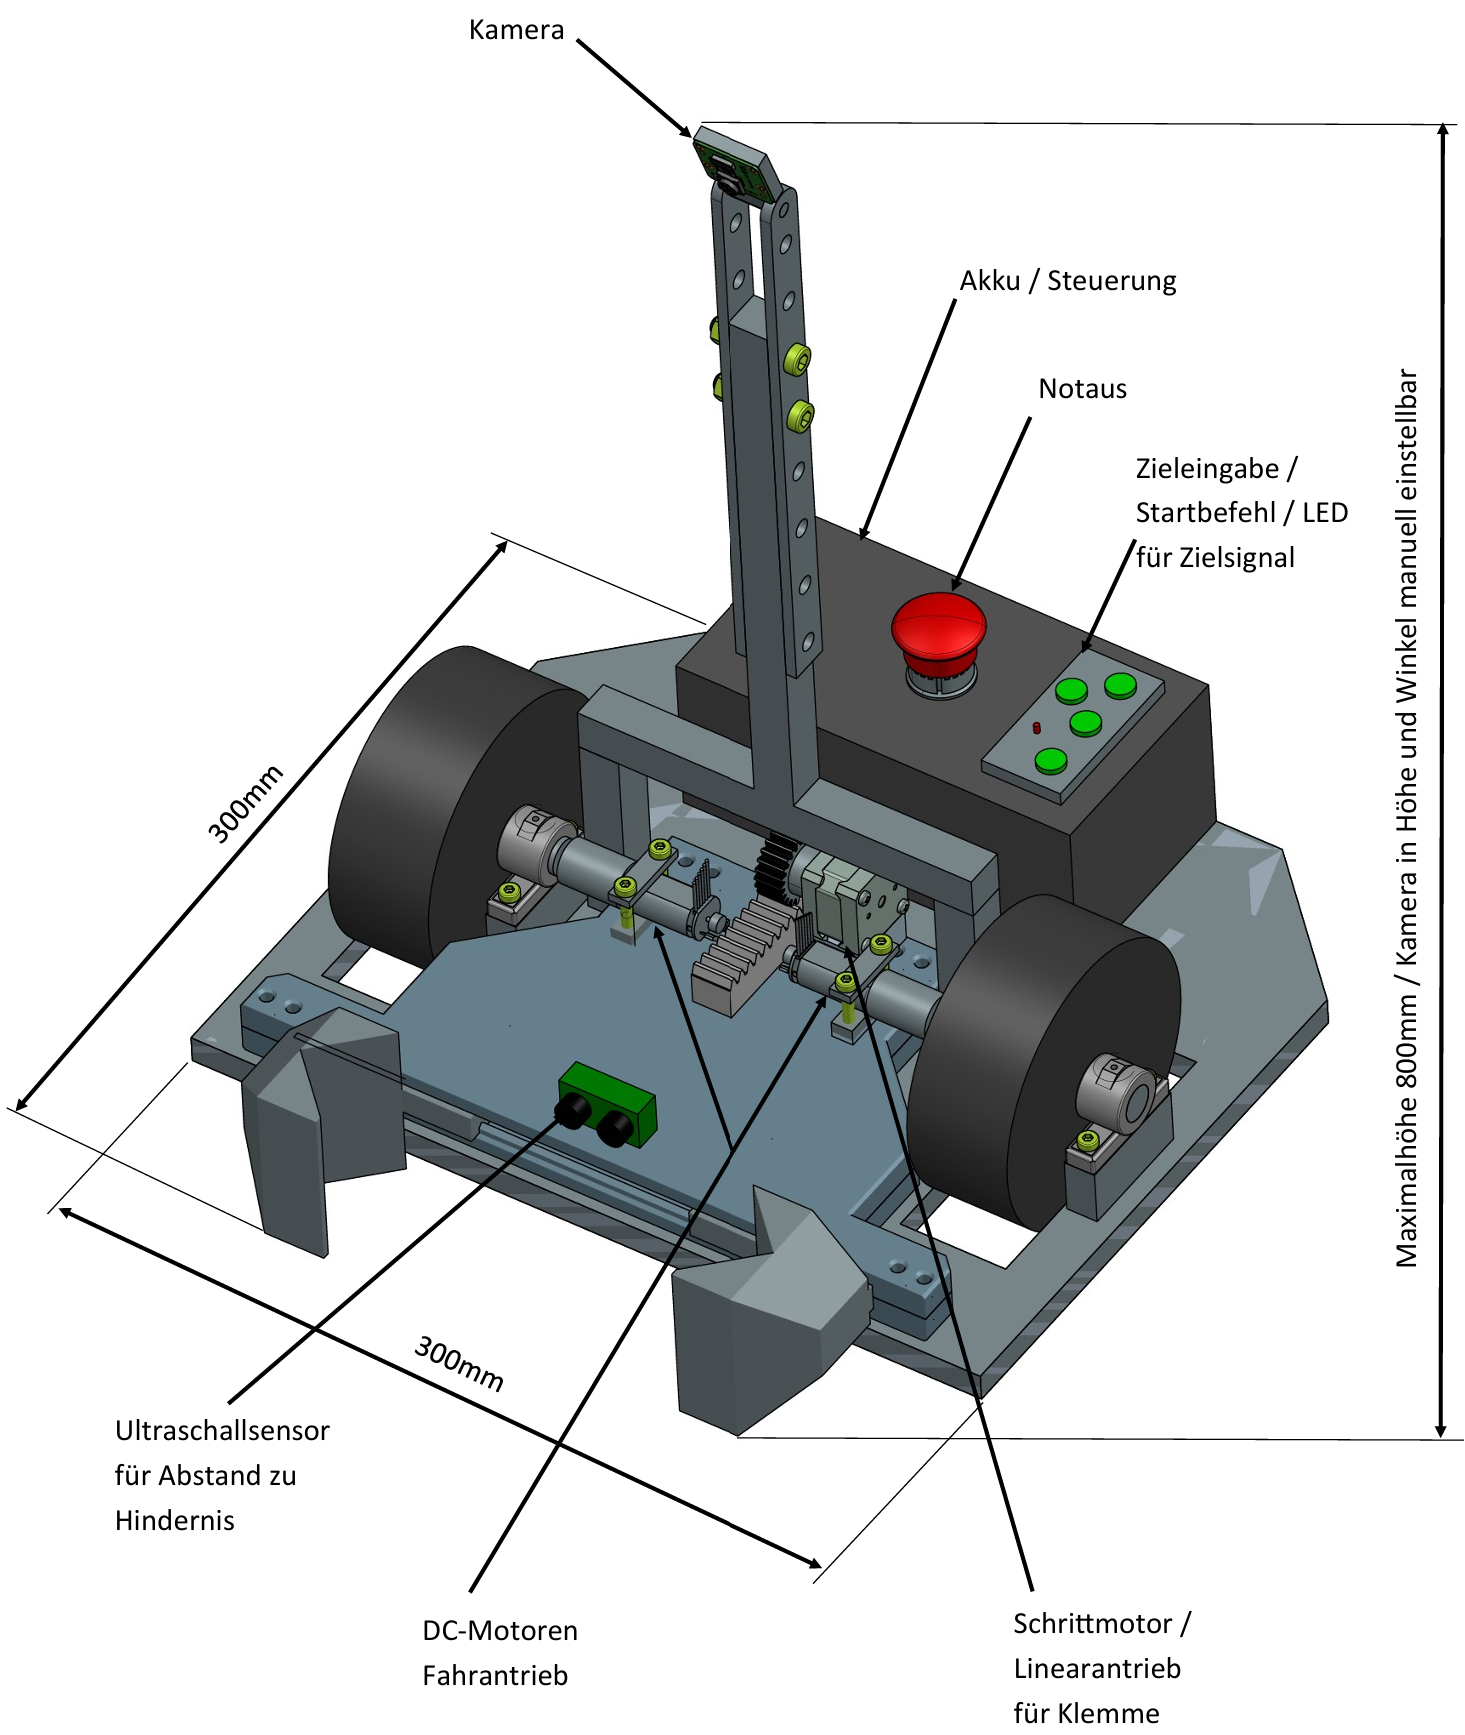
\includegraphics[width=0.85\linewidth]{img/lösungskonzpet/Skizzen/Skizze_Konzept_beschriftet.png}
\caption{Skizze des Lösungskonzepts}
\label{img:Konzept-Skizze_Fahrzeug}
\end{figure}

\subsection{Aufbau}

\textbf{TODO:} 
- Aufbau mit fehlenden Daten ergänzen.  


Der Roboter besteht aus zwei (TODO welche) Rädern, die mit jeweils einem DC-Motor angetrieben werden.

Die Raspberry Pi Camera Module 3 Kamera befindet sich auf einem höhenverstellbaren Masten. Die Höhe der Kamera kann zwischen 40 und 60 Zentimeter variabel eingestellt werden. Der Winkel der Kamera kann ebenfalls verändert werden. Somit kann die Kamera-Position im späteren Verlauf des Projektes einfach optimiert werden.

Zur Hindernisbewältigung befinden sich an der Vorderseite des Roboters zwei Klemmblöcke mit einem Abstand von (TODO: Abstand einfügen) zueinander. Ein Schrittmotor kann diese Klemmblöcke zusammenziehen, um ein Hindernis aufzuheben. Damit der Abstand zu einem Hindernis erkannt werden kann, befindet sich ein Ultraschallsensor zwischen den beiden Klemmblöcken. 

Die Motoren, Sensoren und Eingabeknöpfe sind mit einem TinyK22 verbunden.
Das TinyK22 sowie die Kamera sind an einem Raspberry Pi 5 angeschlossen.

Die Energieversorgung für alle Komponenten wird mit einem LiPo-Akku sichergestellt (Begründung im Anhang \ref{a3:Energiequelle}).
Mit dem Notaus-Knopf kann die Energieversorgung zu allen Komponenten direkt unterbrochen werden.

\subsection{Ablauf}

Im Ablaufdiagramm (Abbildung \ref{img:ablaufdiagramm}) wird der Ablauf des Roboters von Start bis Ziel übersichtlich aufgezeigt.

\begin{figure}[H]
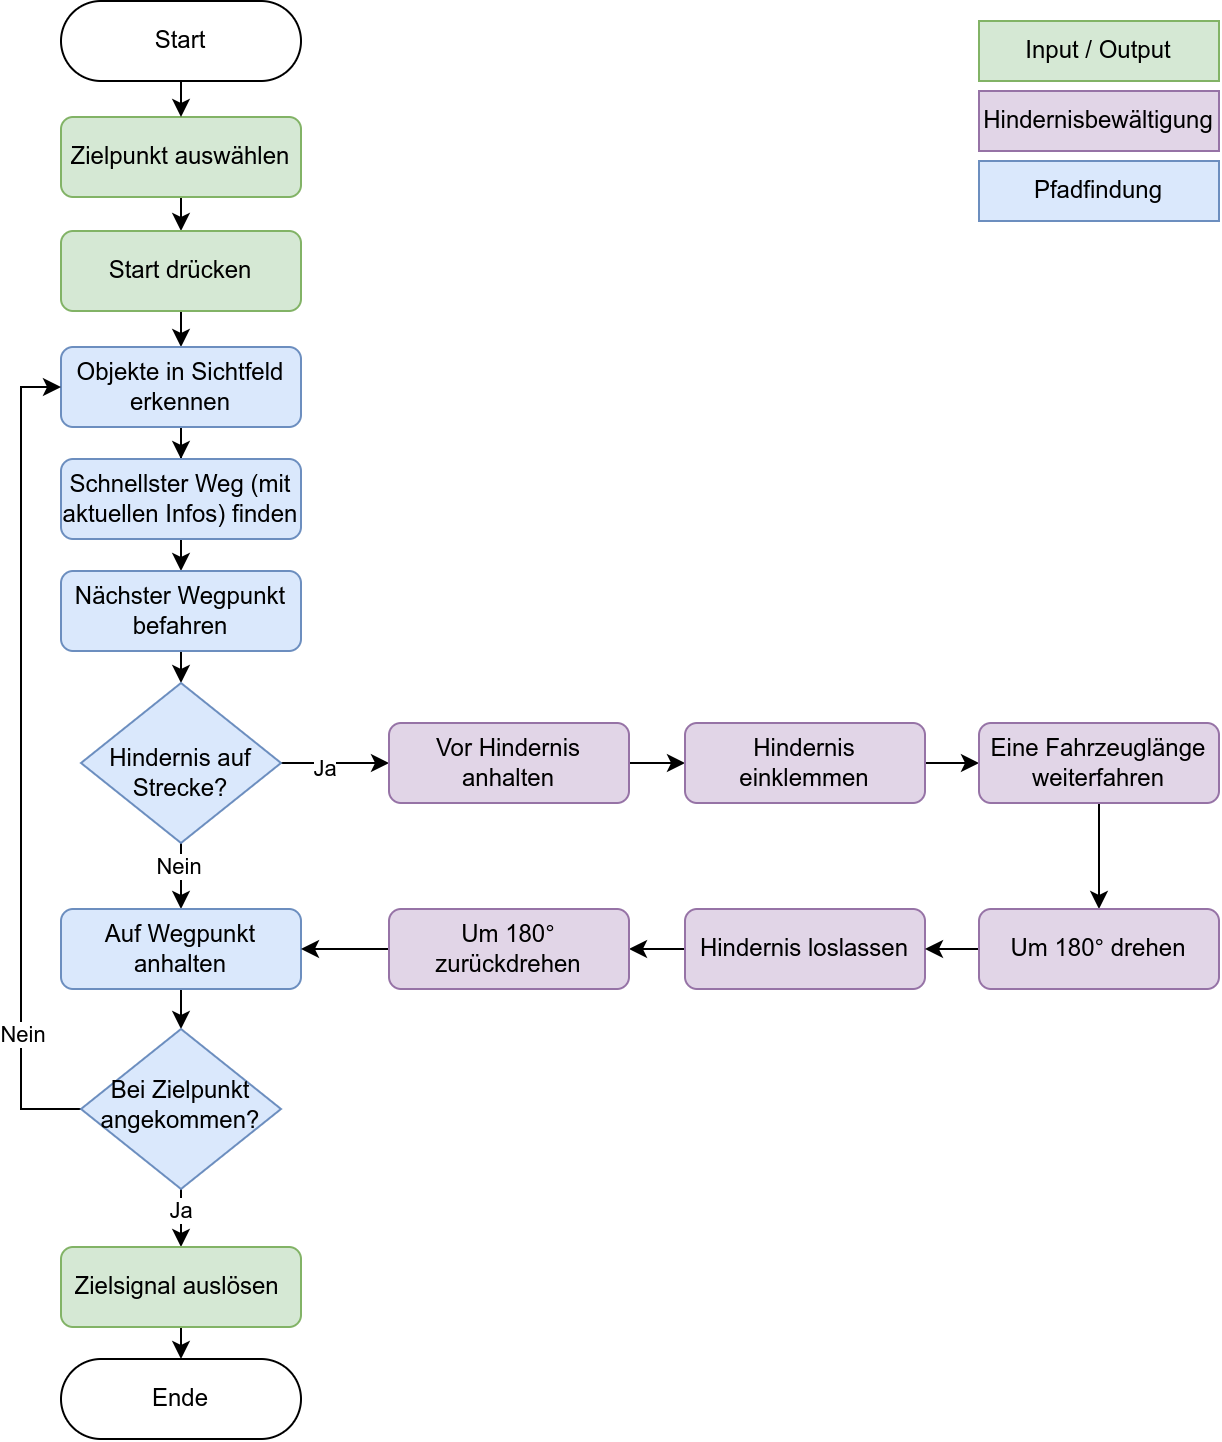
\includegraphics[width=0.9\textwidth]{img/lösungskonzpet/Ablaufdiagramm.png}
\caption{Ablaufdiagramm}
\label{img:ablaufdiagramm}
\end{figure}

\newpage
\subsection{Zielauswahl}
\imagefloat{img/lösungskonzpet/Skizzen/Zielauswahl.png}{Zielauswahl (Ausschnitt Abbildung \ref{img:Konzept-Skizze_Fahrzeug})}{0.3\textwidth}

Das Ziel des Roboters muss vor dem Start ausgewählt werden. Die Auswahlmöglichkeiten sind A, B oder C. Jede dieser Optionen kann über einen physischen Knopf am Roboter festgelegt werden.

Neben der Zielauswahl befindet sich der Knopf zum Starten des Fahrzeugs. Dieser funktioniert erst, wenn ein Ziel ausgewählt wurde. Bei einer mehrfachen Zielauswahl wird das zuletzt gewählte Ziel angesteuert.

Sobald der Roboter im Ziel angekommen ist, erleuchtet die LED, welche sich neben dem Start-Knopf befindet. 

\subsection{Fortbewegung} 

Die Fortbewegung wird nach dem Prinzip Roomba realisiert. Wie der Name schon erahnen lässt, handelt es sich dabei um ein ähnliches System, wie wir es von Staubsauger-Robotern kennen. Das Prinzip besteht aus zwei einzeln angetriebenen Rädern und einem Stützelement. Die angetriebenen Räder können unabhängig in beide Drehrichtungen angetrieben werden, wodurch ein Wenden an Ort und Stelle ermöglicht wird. Die beiden Räder sind in Längsrichtung zentrisch angeordnet, damit sich das Fahrzeug um den eigenen Mittelpunkt drehen kann, ohne dass ein Versatz entsteht. Weitere Details dazu befinden sich im Anhang unter \ref{a3:}

Als Antriebsmotoren werden Brushed-DC-Motoren verwendet, die über eine H-Brücke mit einem PWM-Signal angesteuert werden können. Jeder Motor verfügt über einen Encoder, der überwacht, dass beide Motoren die gleiche Anzahl an Umdrehungen ausführen. Gesteuert werden die Motoren von einem TinyK22 (wieso der TinyK22 gewählt wurde, siehe Anhang \ref{a3:Hardware Steuerung}), der die H-Brücke ansteuert. Weitere Details können im Anhang, unter \ref{a3:Fahrantrieb} und \ref{a3:Sensorik:Positionsabfrage} nachgeschlagen werden.
\newpage
Der TinyK22 ist über eine UART-Schnittstelle mit dem Raspberry Pi verbunden (siehe Abbildung \ref{img:UART_Schnittstelle}). Zunächst sendet der TinyK22 das gewünschte Ziel an den Raspberry Pi. Der Raspberry Pi wertet mit der Kamera aus, welches der nächste beste Punkt ohne Pylone ist und teilt anschliessend dem TinyK22 mit, um welchen Winkel das Fahrzeug ausgerichtet werden muss, um diesen Punkt zu erreichen. Somit dreht sich das Fahrzeug auf die angepeilte Linie, dies wird vom Liniensensor darauf erkannt. Wird die Linie nicht erkannt, sucht das System diese durch Drehungen im Bereich von ±15 Grad. Sobald die Linie gefunden wird, meldet der TinyK22 dem Raspberry Pi, wie weit sich das Fahrzeug gedreht hat.

\begin{figure}[H]
\centering
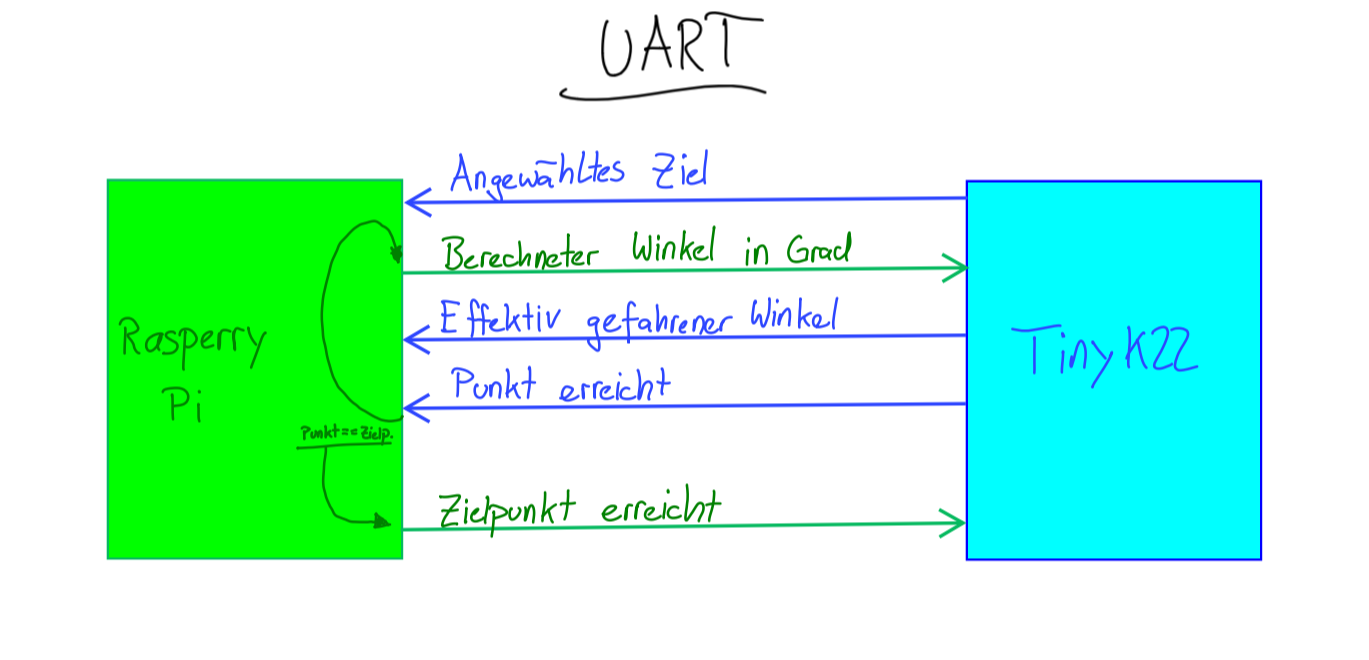
\includegraphics[width=\textwidth]{img/lösungskonzpet/Skizzen/UART_Schnittstelle.png}
\caption{UART Schnittstelle}
\label{img:UART_Schnittstelle}
\end{figure}

Das Fahrzeug folgt der Linie mithilfe des Liniensensors. Erkennt der Sensor eine breitere Linie, also einen Punkt, informiert der TinyK22 den Raspberry Pi, stoppt das Fahrzeug, und der Vorgang beginnt erneut. Sobald das Fahrzeug den Zielpunkt erreicht, signalisiert der Raspberry Pi dies dem TinyK22, der daraufhin eine LED blinken lässt.

\newpage

\subsection{Wegfindung}

Um den schnellsten Weg ins Ziel zu finden, wird der vorgegebene Graph in der Software gespeichert und der kürzeste Weg mittels des Dijkstra-Algorithmus berechnet (siehe Anhang \ref{a3:Wegfindung}). Sobald die Kamera neue Informationen über die Strecke erkennt (siehe \ref{sub:Objekterkennung}), wird der Graph entsprechend angepasst, und der kürzeste Weg wird anhand der aktuellen Position neu berechnet. Ursprünglich haben alle Linien im Graphen eine einheitliche Gewichtung.

Je nach neu erhaltener Information werden folgende Anpassungen am Graphen vorgenommen: \begin{itemize} 
  \item Pylon auf Wegpunkt erkannt: Der Wegpunkt (Knoten) wird aus dem Graphen entfernt.
  \item Linie wurde entfernt: Die Linie (Kante) wird aus dem Graphen entfernt. 
  \item Hindernis auf Linie erkannt: Die Linie (Kante) erhält eine höhere Gewichtung.
\end{itemize}

\subsubsection{Objekterkennung} \label{sub:Objekterkennung}
Die Objekterkennung wird mithilfe einer weitwinkligen Raspberry Pi Camera Module 3 Kamera durchgeführt. Dabei werden Pylonen, Hindernisse und Wegpunkte erkannt. Als Software kommt YOLO zum Einsatz (Anhang \ref{a3:Objekterkennung}). Die erkannten Objekte werden für die Wegfindung genutzt. Das Ziel ist es, von Anfang an möglichst viele Objekte zu erfassen und auszuwerten. Da dies jedoch nicht garantiert werden kann, wird die Objekterkennung bei jedem Wegpunkt durchgeführt. 

\subsection{Hindernisbewältigung}
Der Ultraschallsensor überwacht kontinuierlich, ob sich ein Hindernis auf der Linie befindet (siehe Anhang \ref{a3:Objekterkennung_Sensor}). Sobald ein Hindernis in 30 cm Entfernung detektiert wird, verlangsamt sich das Fahrzeug und fährt langsam darauf zu, bis es zwischen den zwei seitlichen Klemmbacken positioniert ist. Diese Distanz ist vorprogrammiert, und das Fahrzeug hält an. Danach wird der Schrittmotor angesteuert, der das Hindernis ergreift und mit einem Mechanismus anhebt (Anhang \ref{a3:Hindernisbewältigungsantrieb} und \ref{a3:Aufnahme_Hindernis}).
Das Fahrzeug fährt anschliessend eine Fahrzeuglänge vor, wobei die Encodermessung die Distanz überwacht. Danach dreht es sich um 180 Grad, und der Schrittmotor löst die Klemmen. Das Fahrzeug fährt nun ein Stück zurück, um das Hindernis nicht mehr zwischen den Klemmbacken zu haben, und vollzieht eine weitere 180-Grad-Drehung. Abschliessend fährt das Fahrzeug mithilfe des Liniensensors entlang der Linie zum nächsten Punkt(siehe Abbildung \ref{img:Skizze_Hindernisbewältigung}.

\begin{figure}[H]
\centering
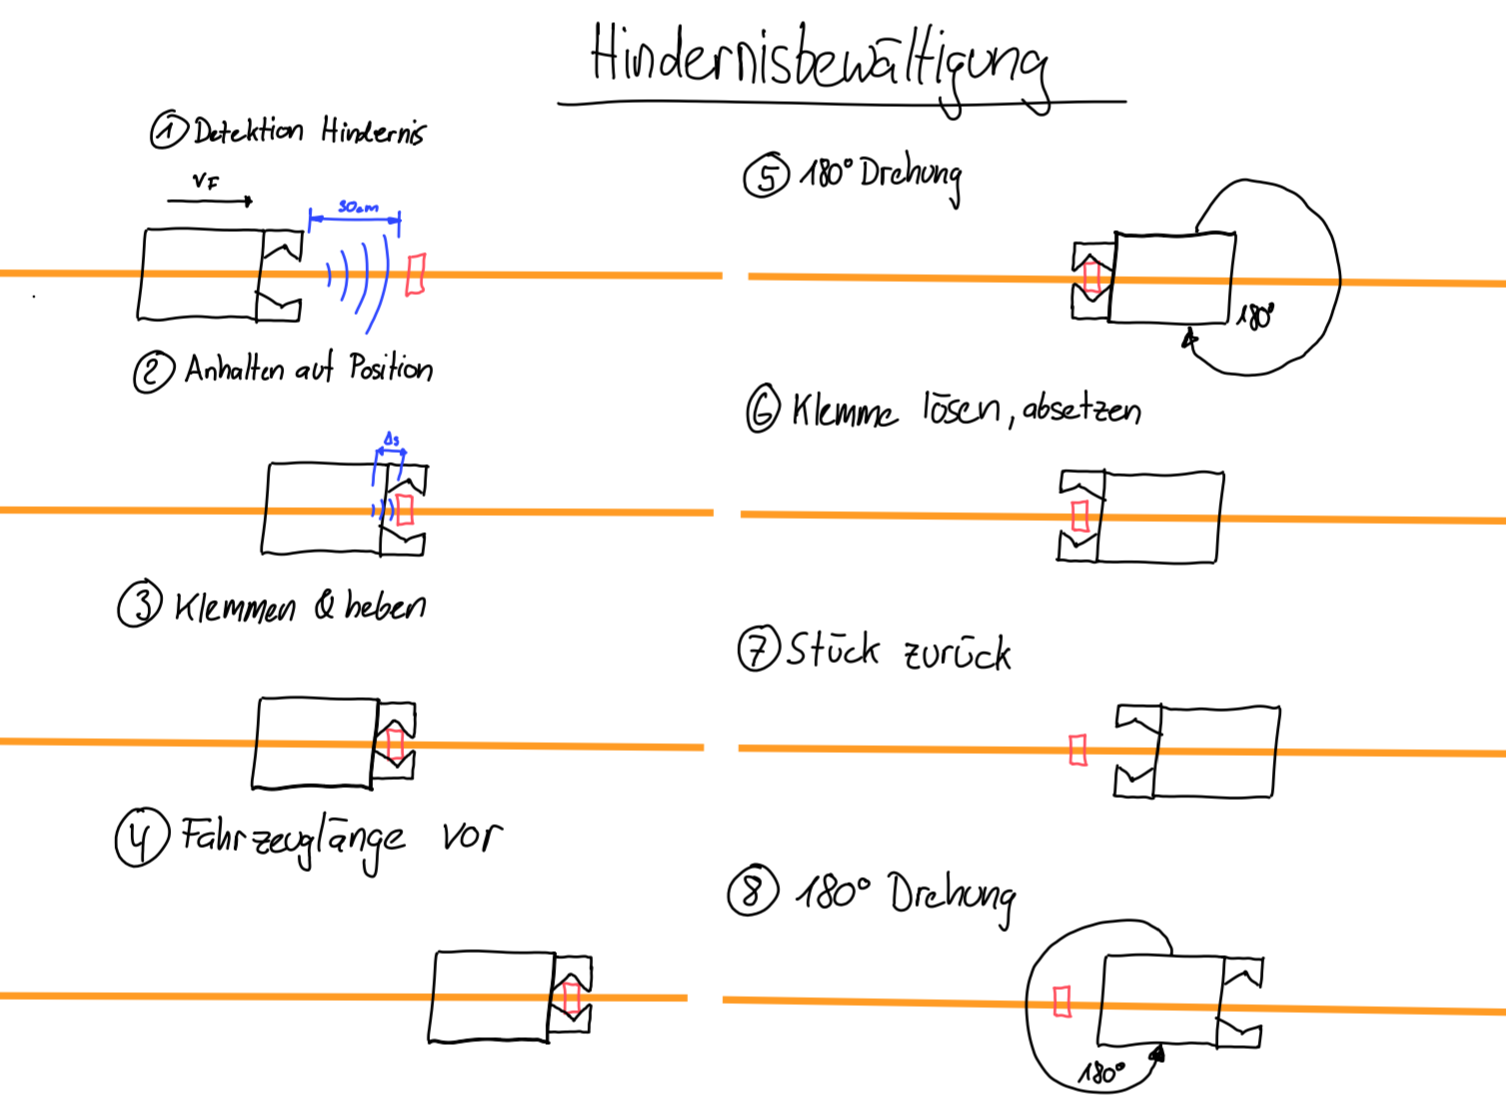
\includegraphics[width=0.8\textwidth]{img/lösungskonzpet/Skizzen/Skizze_Hindernisbewältigung.png}
\caption{Hindernisbewältigung}
\label{img:Skizze_Hindernisbewältigung}
\end{figure}


\subsubsection{Klemmen}
Die Klemmen, die in Punkt 3 und 6 in der Abbildung \ref{img:Skizze_Hindernisbewältigung} benötigt werden erfüllen gleichzeitig mehrere Funktionen.

\begin{enumerate}
    \item Greifen
    \item Anheben
    \item Senken
    \item Loslassen
\end{enumerate}

Alle Funktionen werden mithilfe eines Stepper Motors ausgeübt. Das Design ist in Abbildungen \ref{fig:greifarm_oben} und \ref{fig:greifarm_unten} ersichtlich.
\newline

Zusätzlich soll die Konstruktion helfen, Fehler bei der Messung auszukorrigieren.
\begin{enumerate}
    \item Korrektur-Winkel (bis zu 15°, siehe Kapitel \ref{loes:winkel_verschiebung})
    \item Korrektur Distanz (bis zur Hälfte $b$, was 2.25 cm ist, siehe Kapitel \ref{loes:winkel_verschiebung})
    \item Korrektur Offset (bis zu 2 cm, siehe Kapitel \ref{loes:abstand_klemmen})
\end{enumerate}

\begin{figure}[h!]
    \centering
    % Erste Minipage für das obere Bild
    \begin{minipage}[t]{0.45\textwidth}
        \centering
        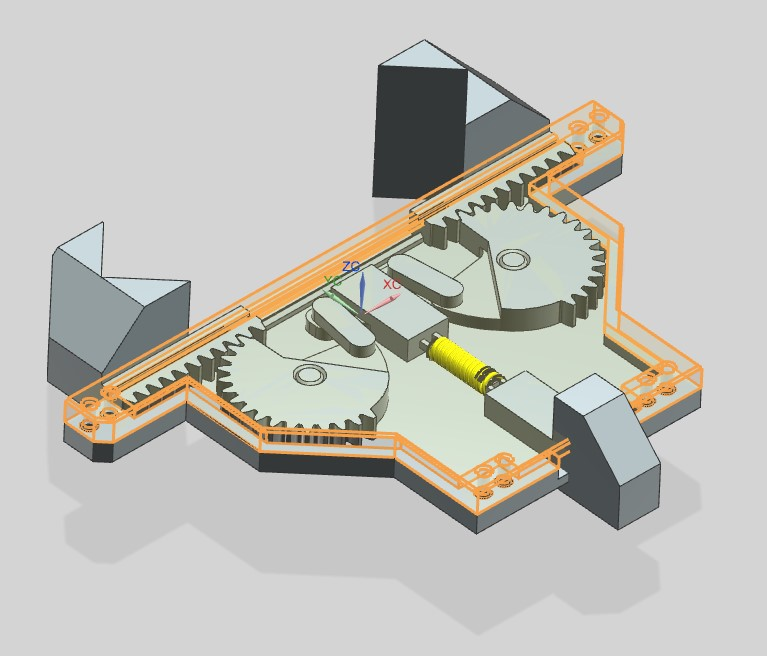
\includegraphics[height=6cm]{img/lösungskonzpet/hindernissaufnahme/Greifarm_oben.jpg}
        \caption{Greifarm oben}
        \label{fig:greifarm_oben}
    \end{minipage}
    \hfill
    % Zweite Minipage für das untere Bild
    \begin{minipage}[t]{0.45\textwidth}
        \centering
        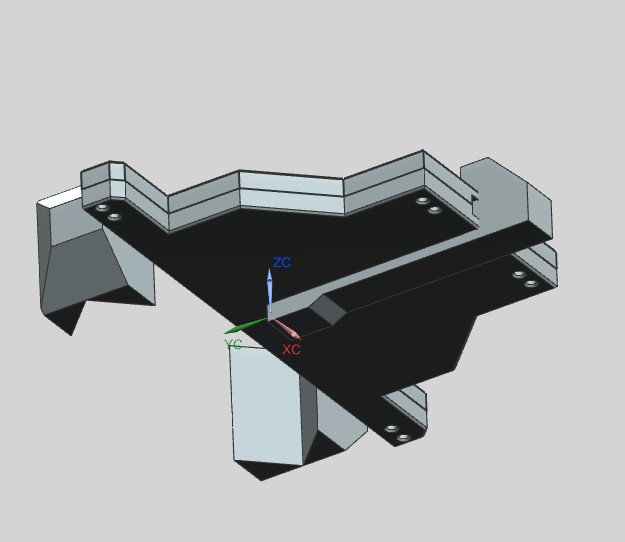
\includegraphics[height=6cm]{img/lösungskonzpet/hindernissaufnahme/Greifarm_unten.jpg}
        \caption{Greifarm unten}
        \label{fig:greifarm_unten}
    \end{minipage}
\end{figure}

Ersichtlich in Abbildung \ref{fig:greifarm_oben} sind die Klemmen, die durch Zahnräder angetrieben werden, welche wiederum von einem linearen Mechanismus bewegt werden, um gleichzeitig den Hebemechanismus auszulösen. Die Feder sorgt dafür, dass, sobald die nötige Griffkraft erreicht ist, weiterhin eine Bewegung für den Hebemechanismus ermöglicht wird. In Abbildung \ref{fig:greifarm_unten} ist der Hebemechanismus zu sehen, der sich von einer Plattform (nicht im Bild sichtbar) abdrückt. An den Rändern befinden sich acht Löcher, von denen vier für Schrauben und die anderen vier für Führungen genutzt werden, um eine kontrollierte Anhebung des Greifarms durch den Mechanismus sicherzustellen.
Der Stepper Motor, der den ganzen Mechanismus antreibt, würde sich auf dem Gehäuse befinden. Dieser Mechanismus wurde dafür ausgelegt, um von Hand betrieben zu werden (für Tests). Die Tests des Mechanismus sind im Kapitel \ref{} ersichtlich.

\end{document}